\subsubsection{Giao diện Admin - Quản lý người dùng}

Tương tự với trang quản lý công ty và quản lý công việc, trang quản lý người dùng cũng sử dụng các loại truy vấn sau để hỗ trợ cho các thao tác CRUD:

\begin{itemize}
    \item \textbf{Query with single/composite condition}: Để fetch lên dữ liệu toàn bộ người dùng trong hệ thống theo cơ chế phân trang và một số điều kiện như \textbf{Tên người dùng}, \textbf{Email}
    \begin{figure}[H]
        \centering
        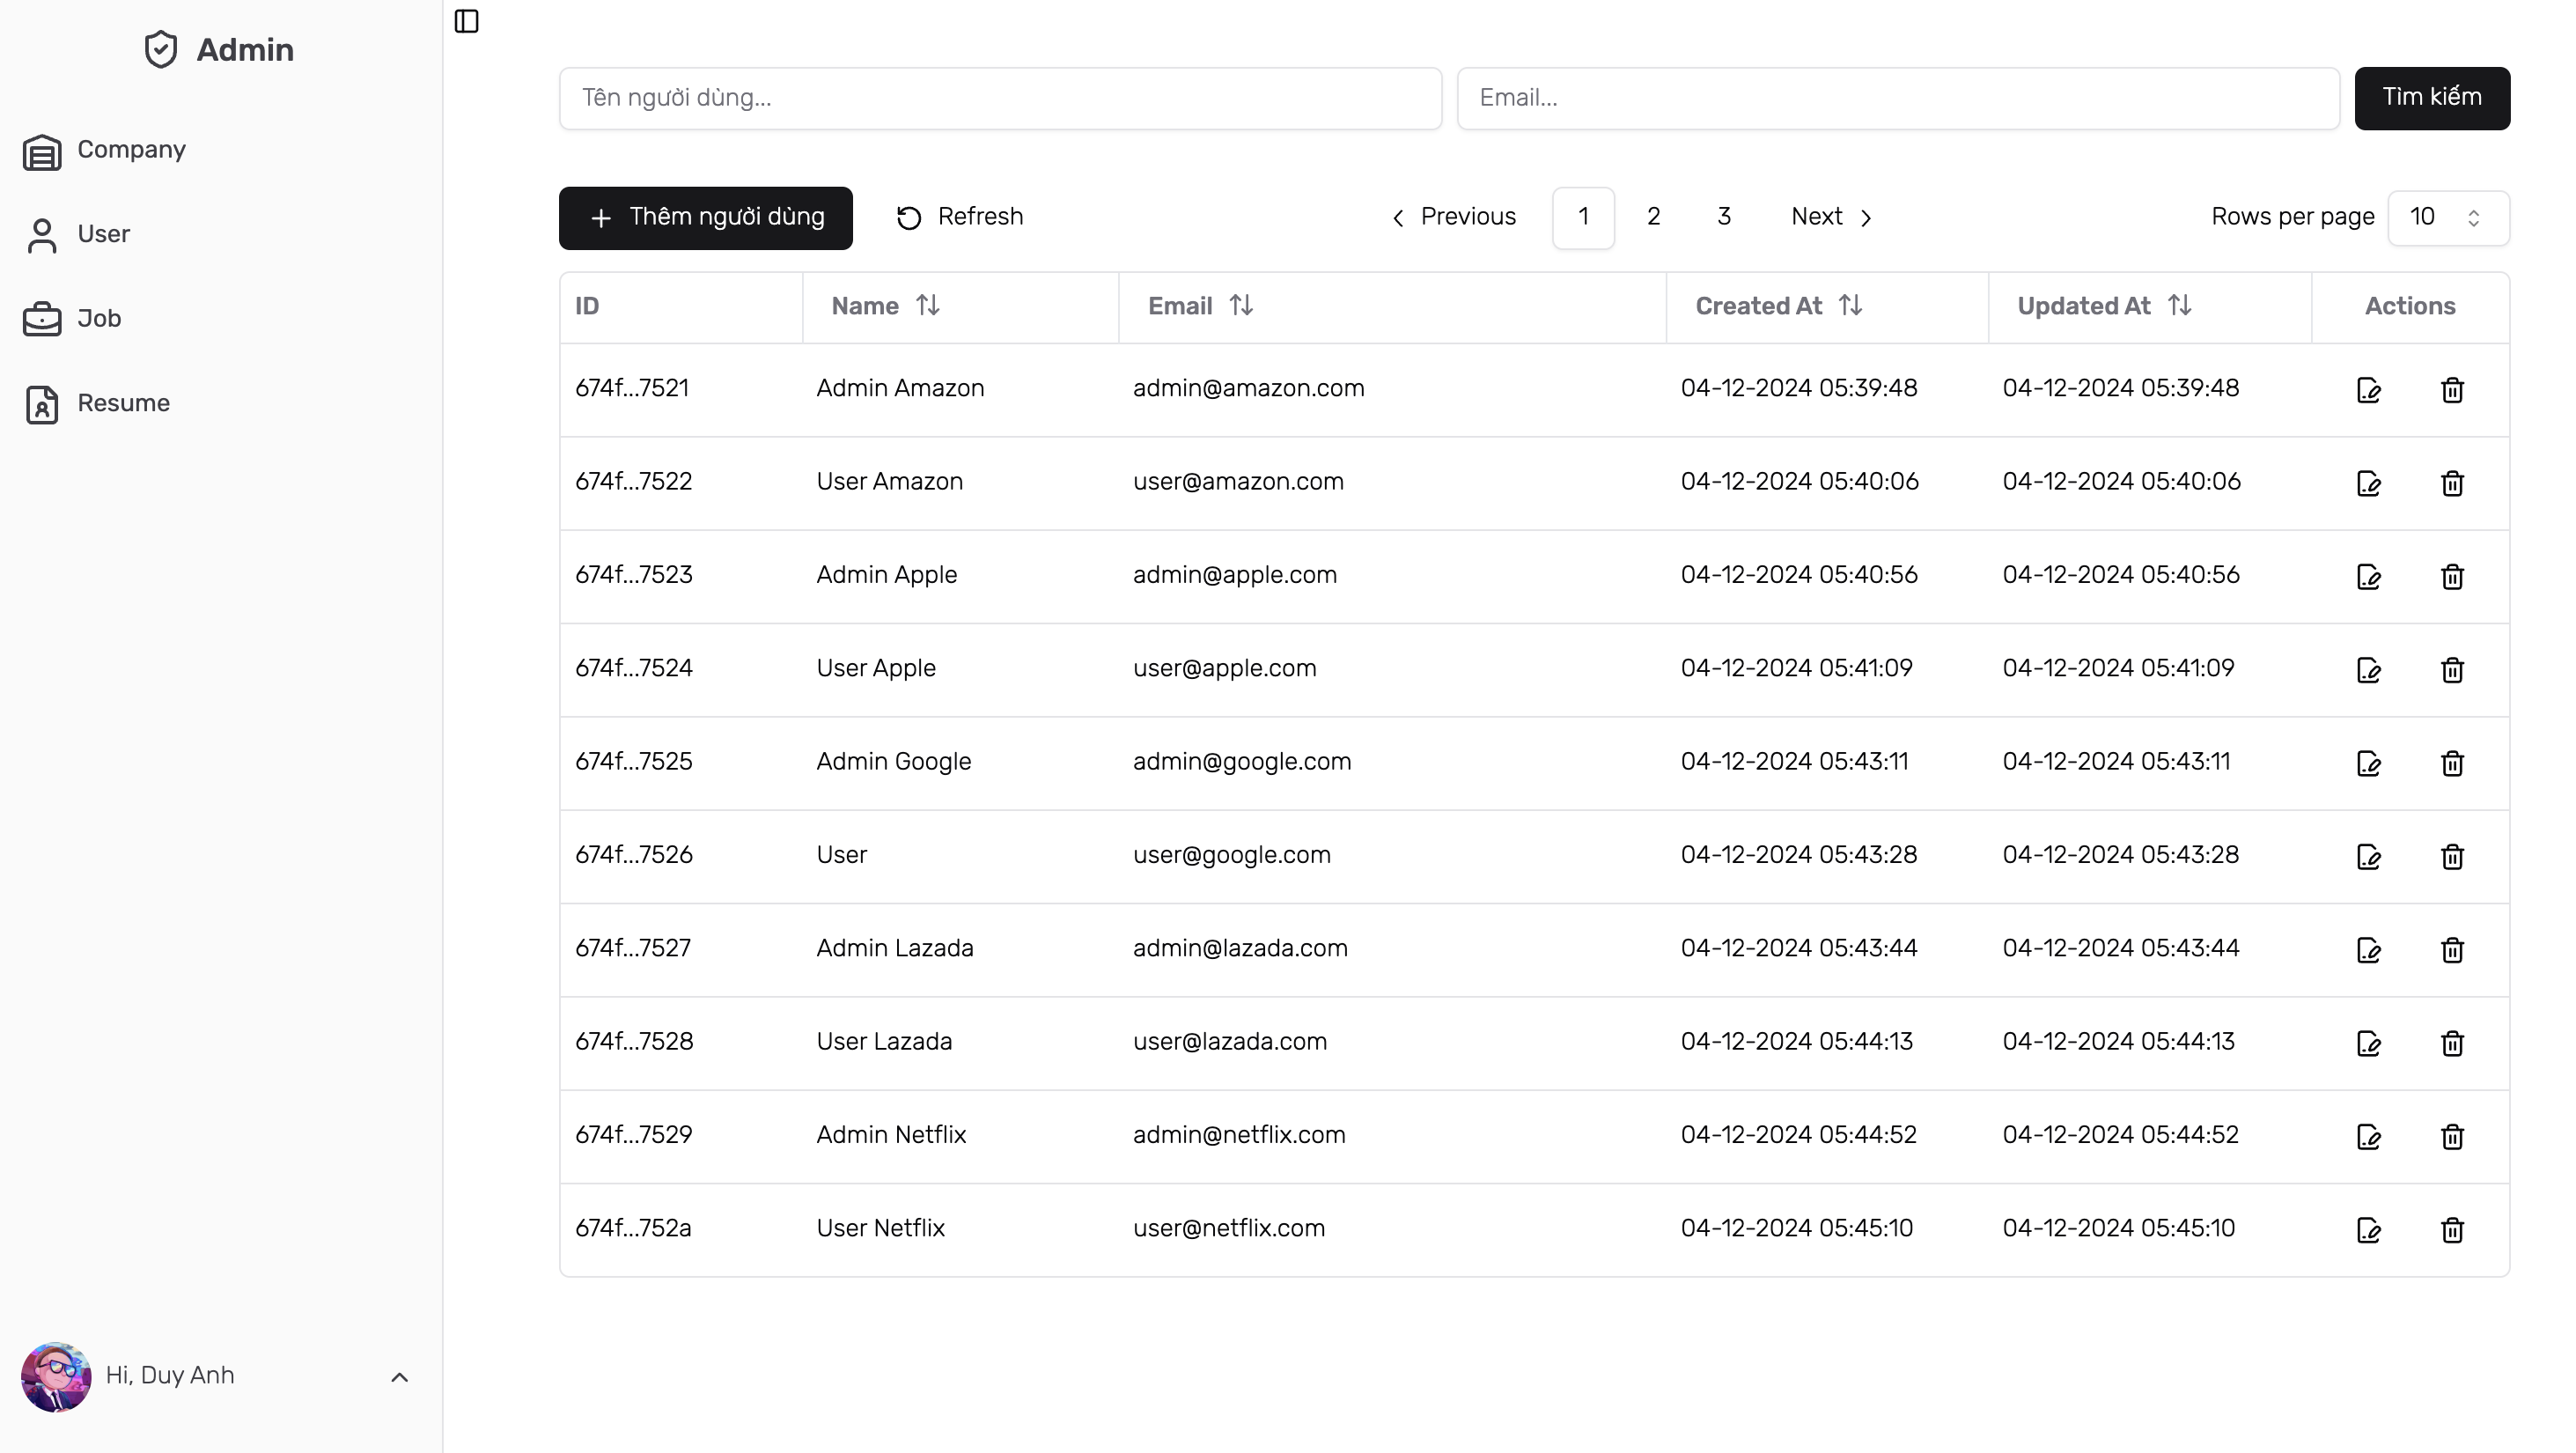
\includegraphics[width=\linewidth]{DBMS-Application/Images/admin-user.png}
        \caption{Trang quản lý người dùng - Danh sách người dùng trong hệ thống}
        \label{fig:enter-label}
    \end{figure}
    
    \item \textbf{Insert}: Thêm mới một người dùng
    \begin{figure}[H]
        \centering
        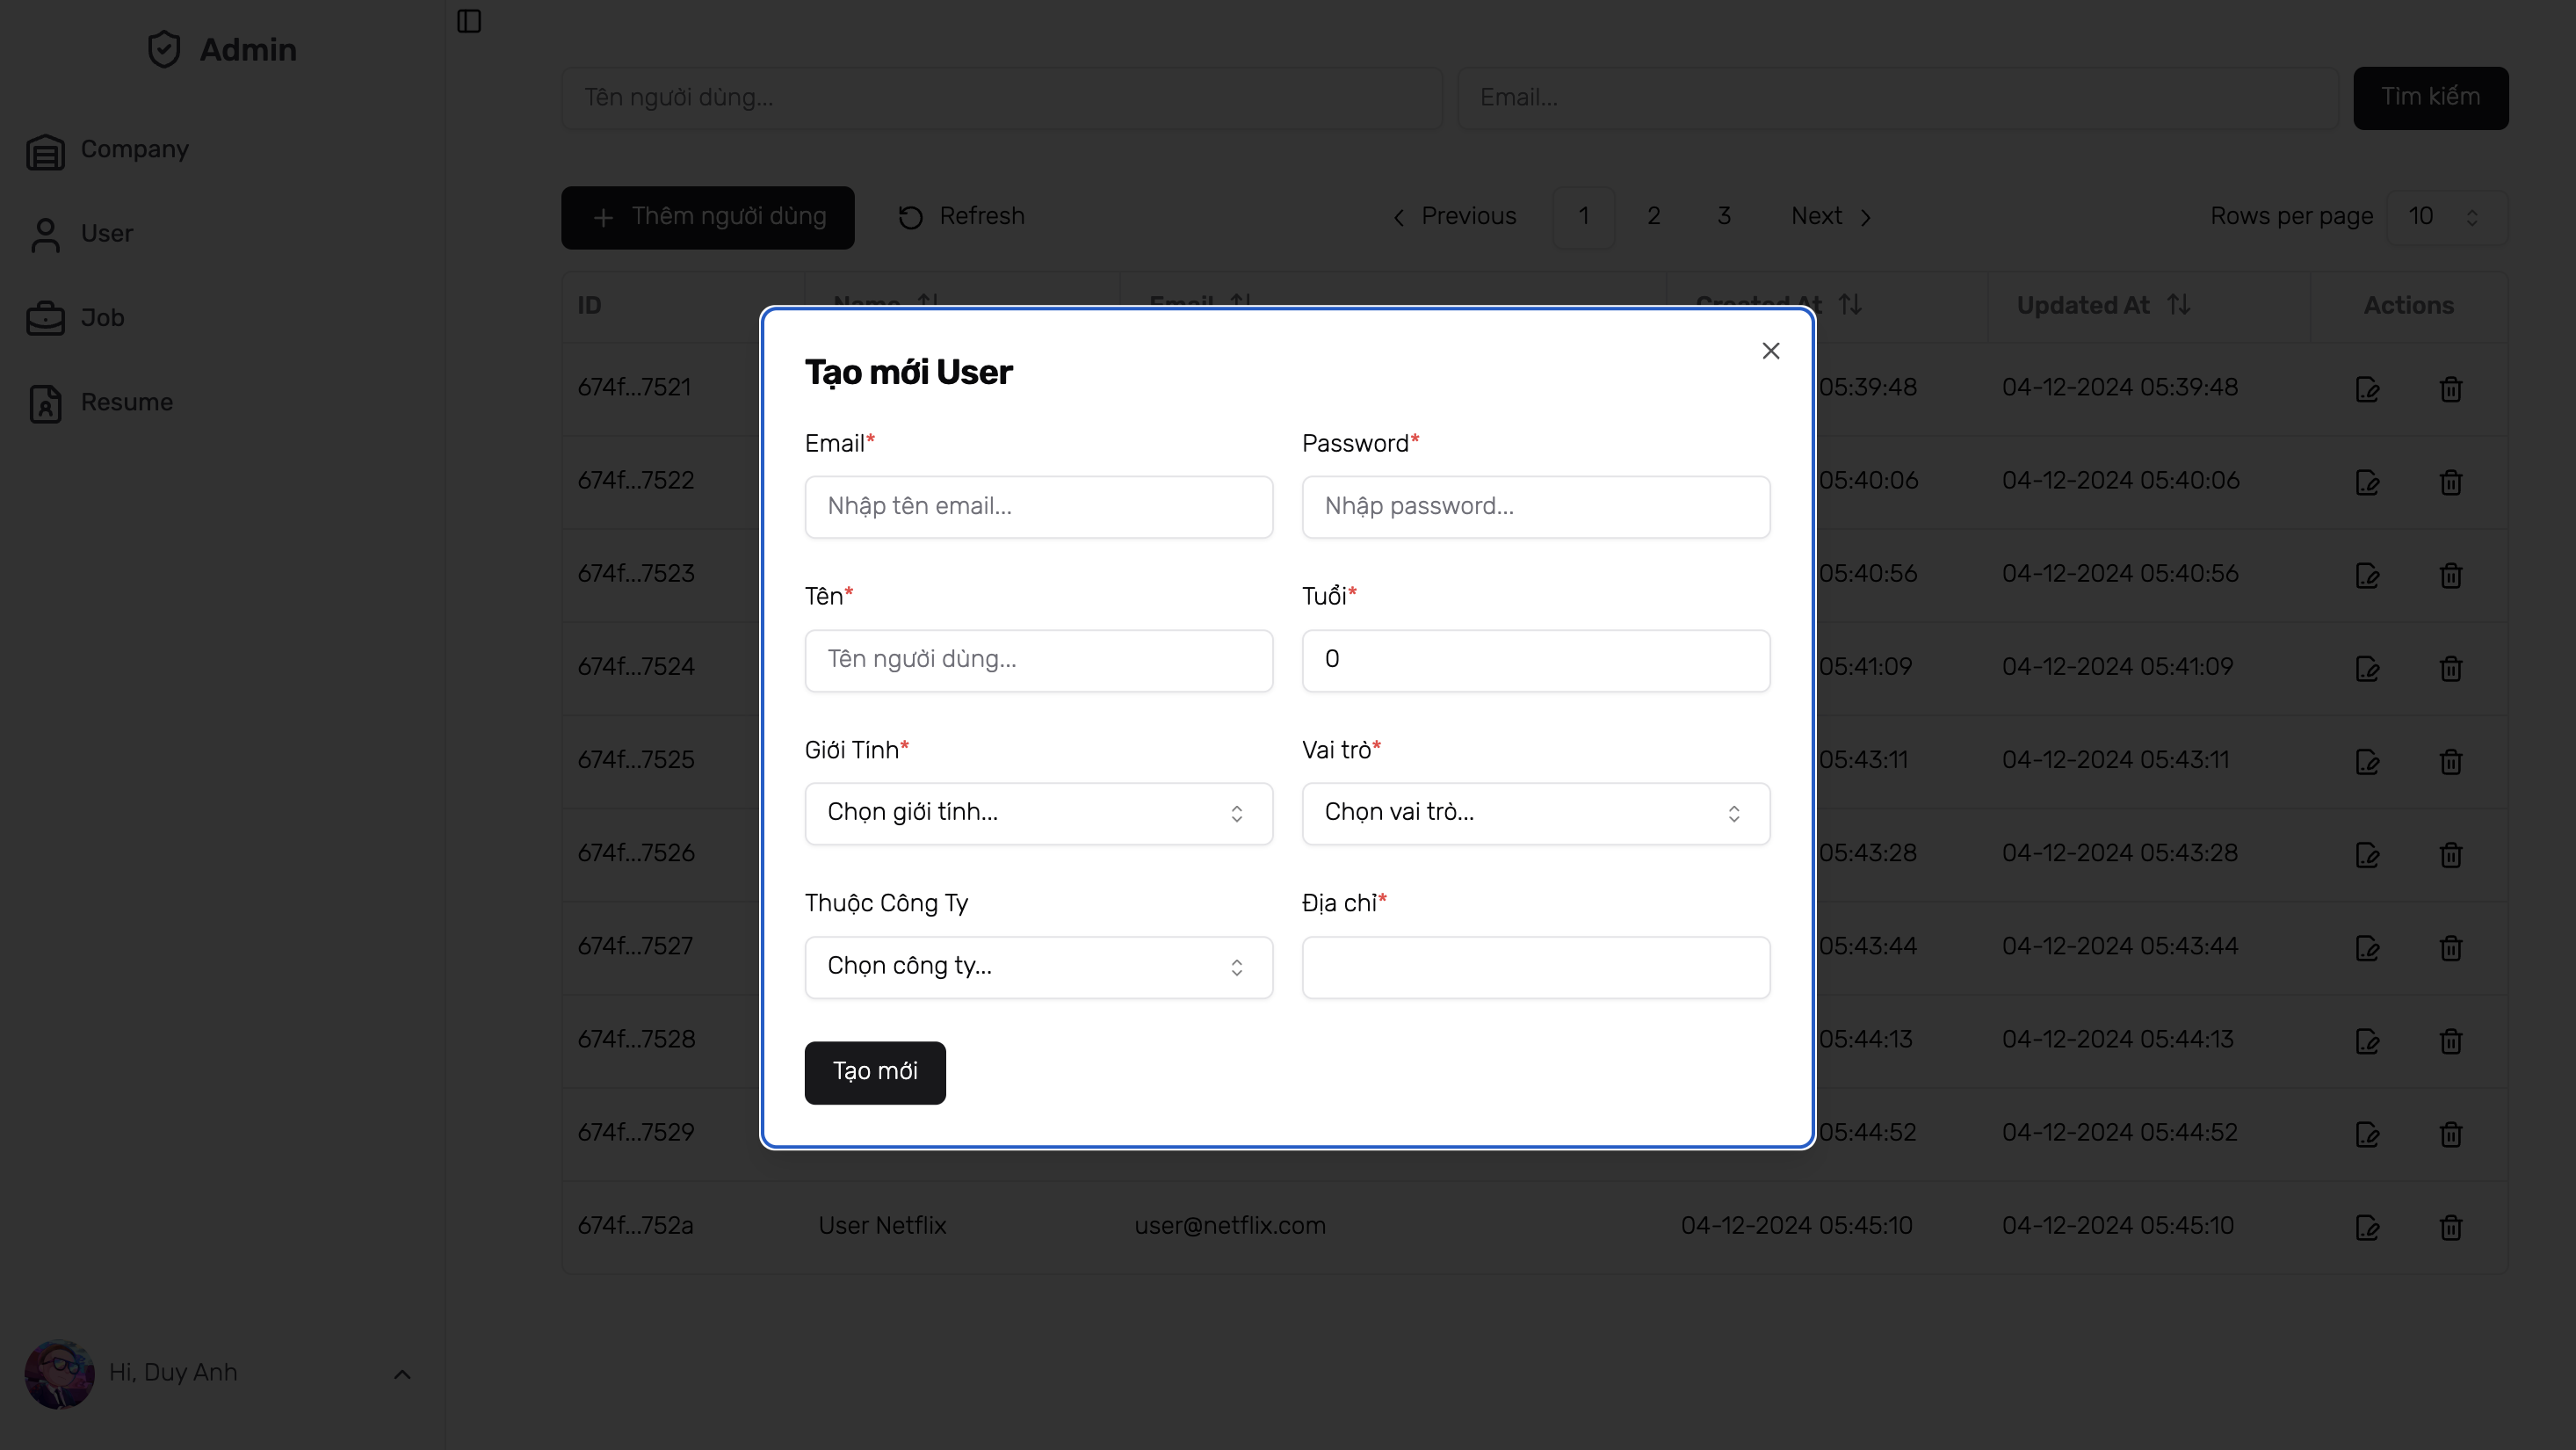
\includegraphics[width=\linewidth]{DBMS-Application/Images/create-user.png}
        \caption{Trang quản lý người dùng - Thêm mới người dùng}
        \label{fig:enter-label}
    \end{figure}

    \item \textbf{Update}: Cập nhật/chỉnh sửa thông tin người dùng cụ thể
    \begin{figure}[H]
        \centering
        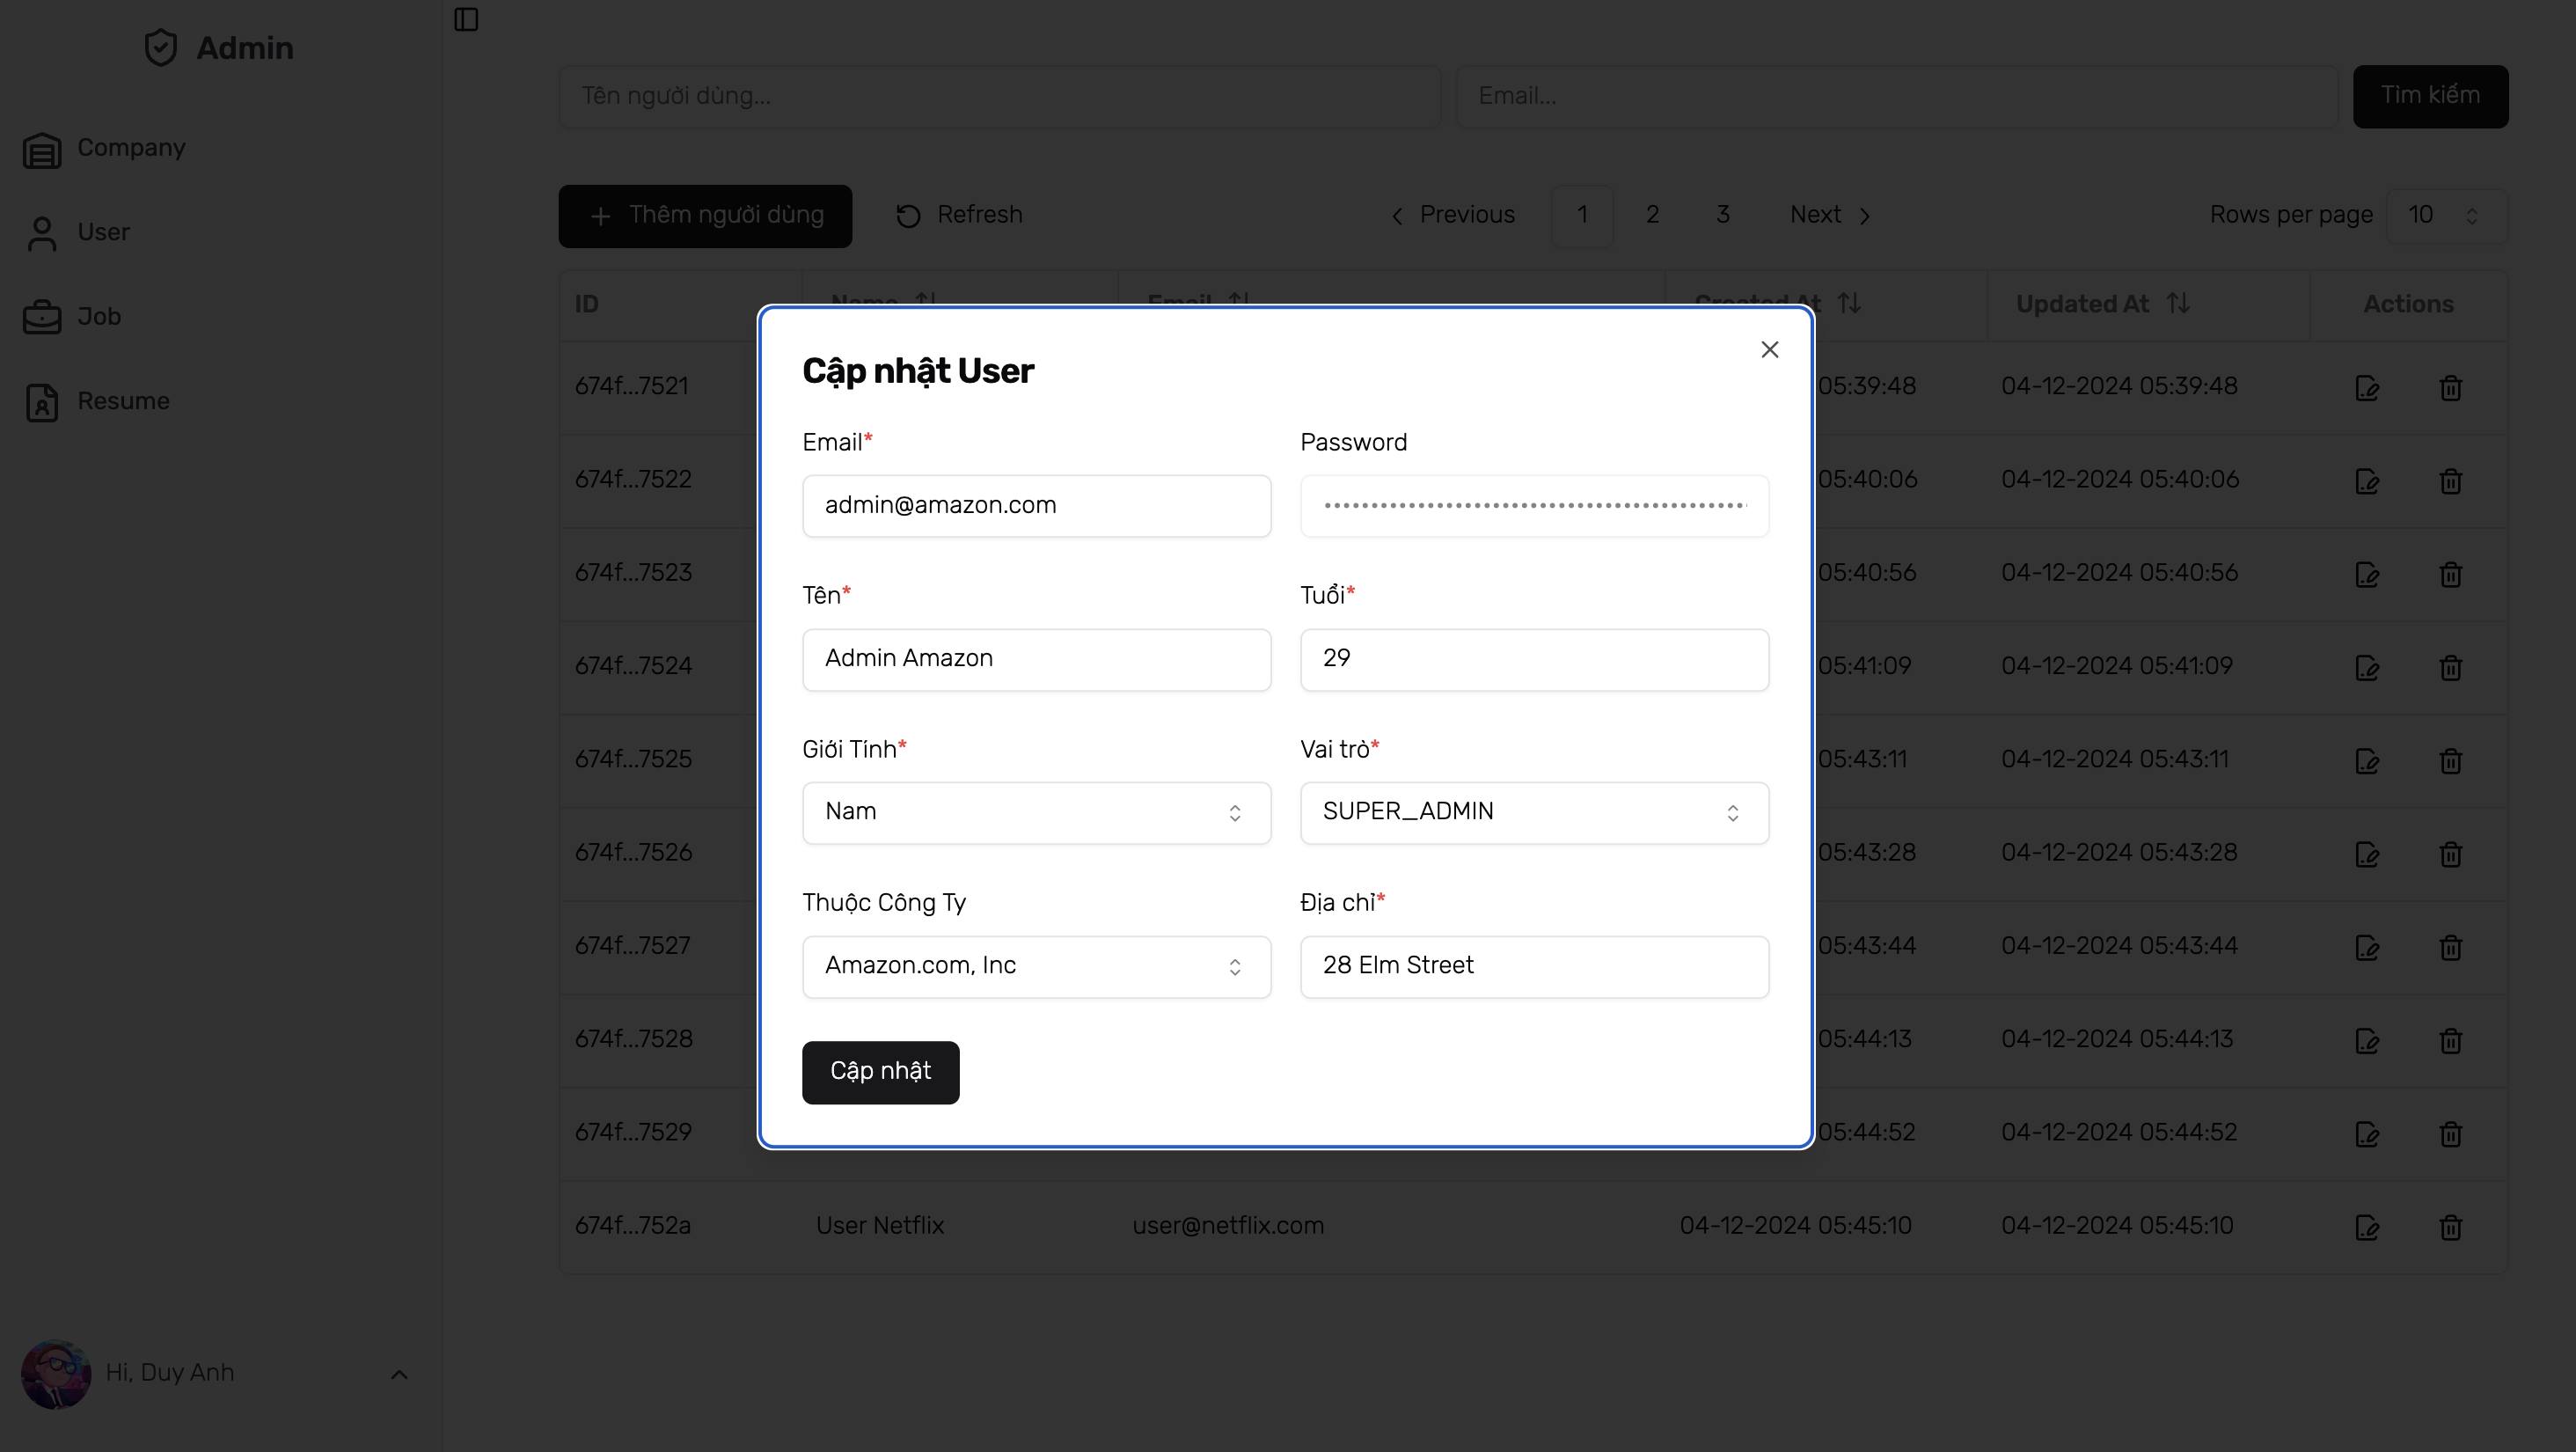
\includegraphics[width=\linewidth]{DBMS-Application/Images/update-user.png}
        \caption{Trang quản lý người dùng - Cập nhật thông tin người dùng}
        \label{fig:enter-label}
    \end{figure}

    \item \textbf{Delete}: Xoá người dùng
    \begin{figure}[H]
        \centering
        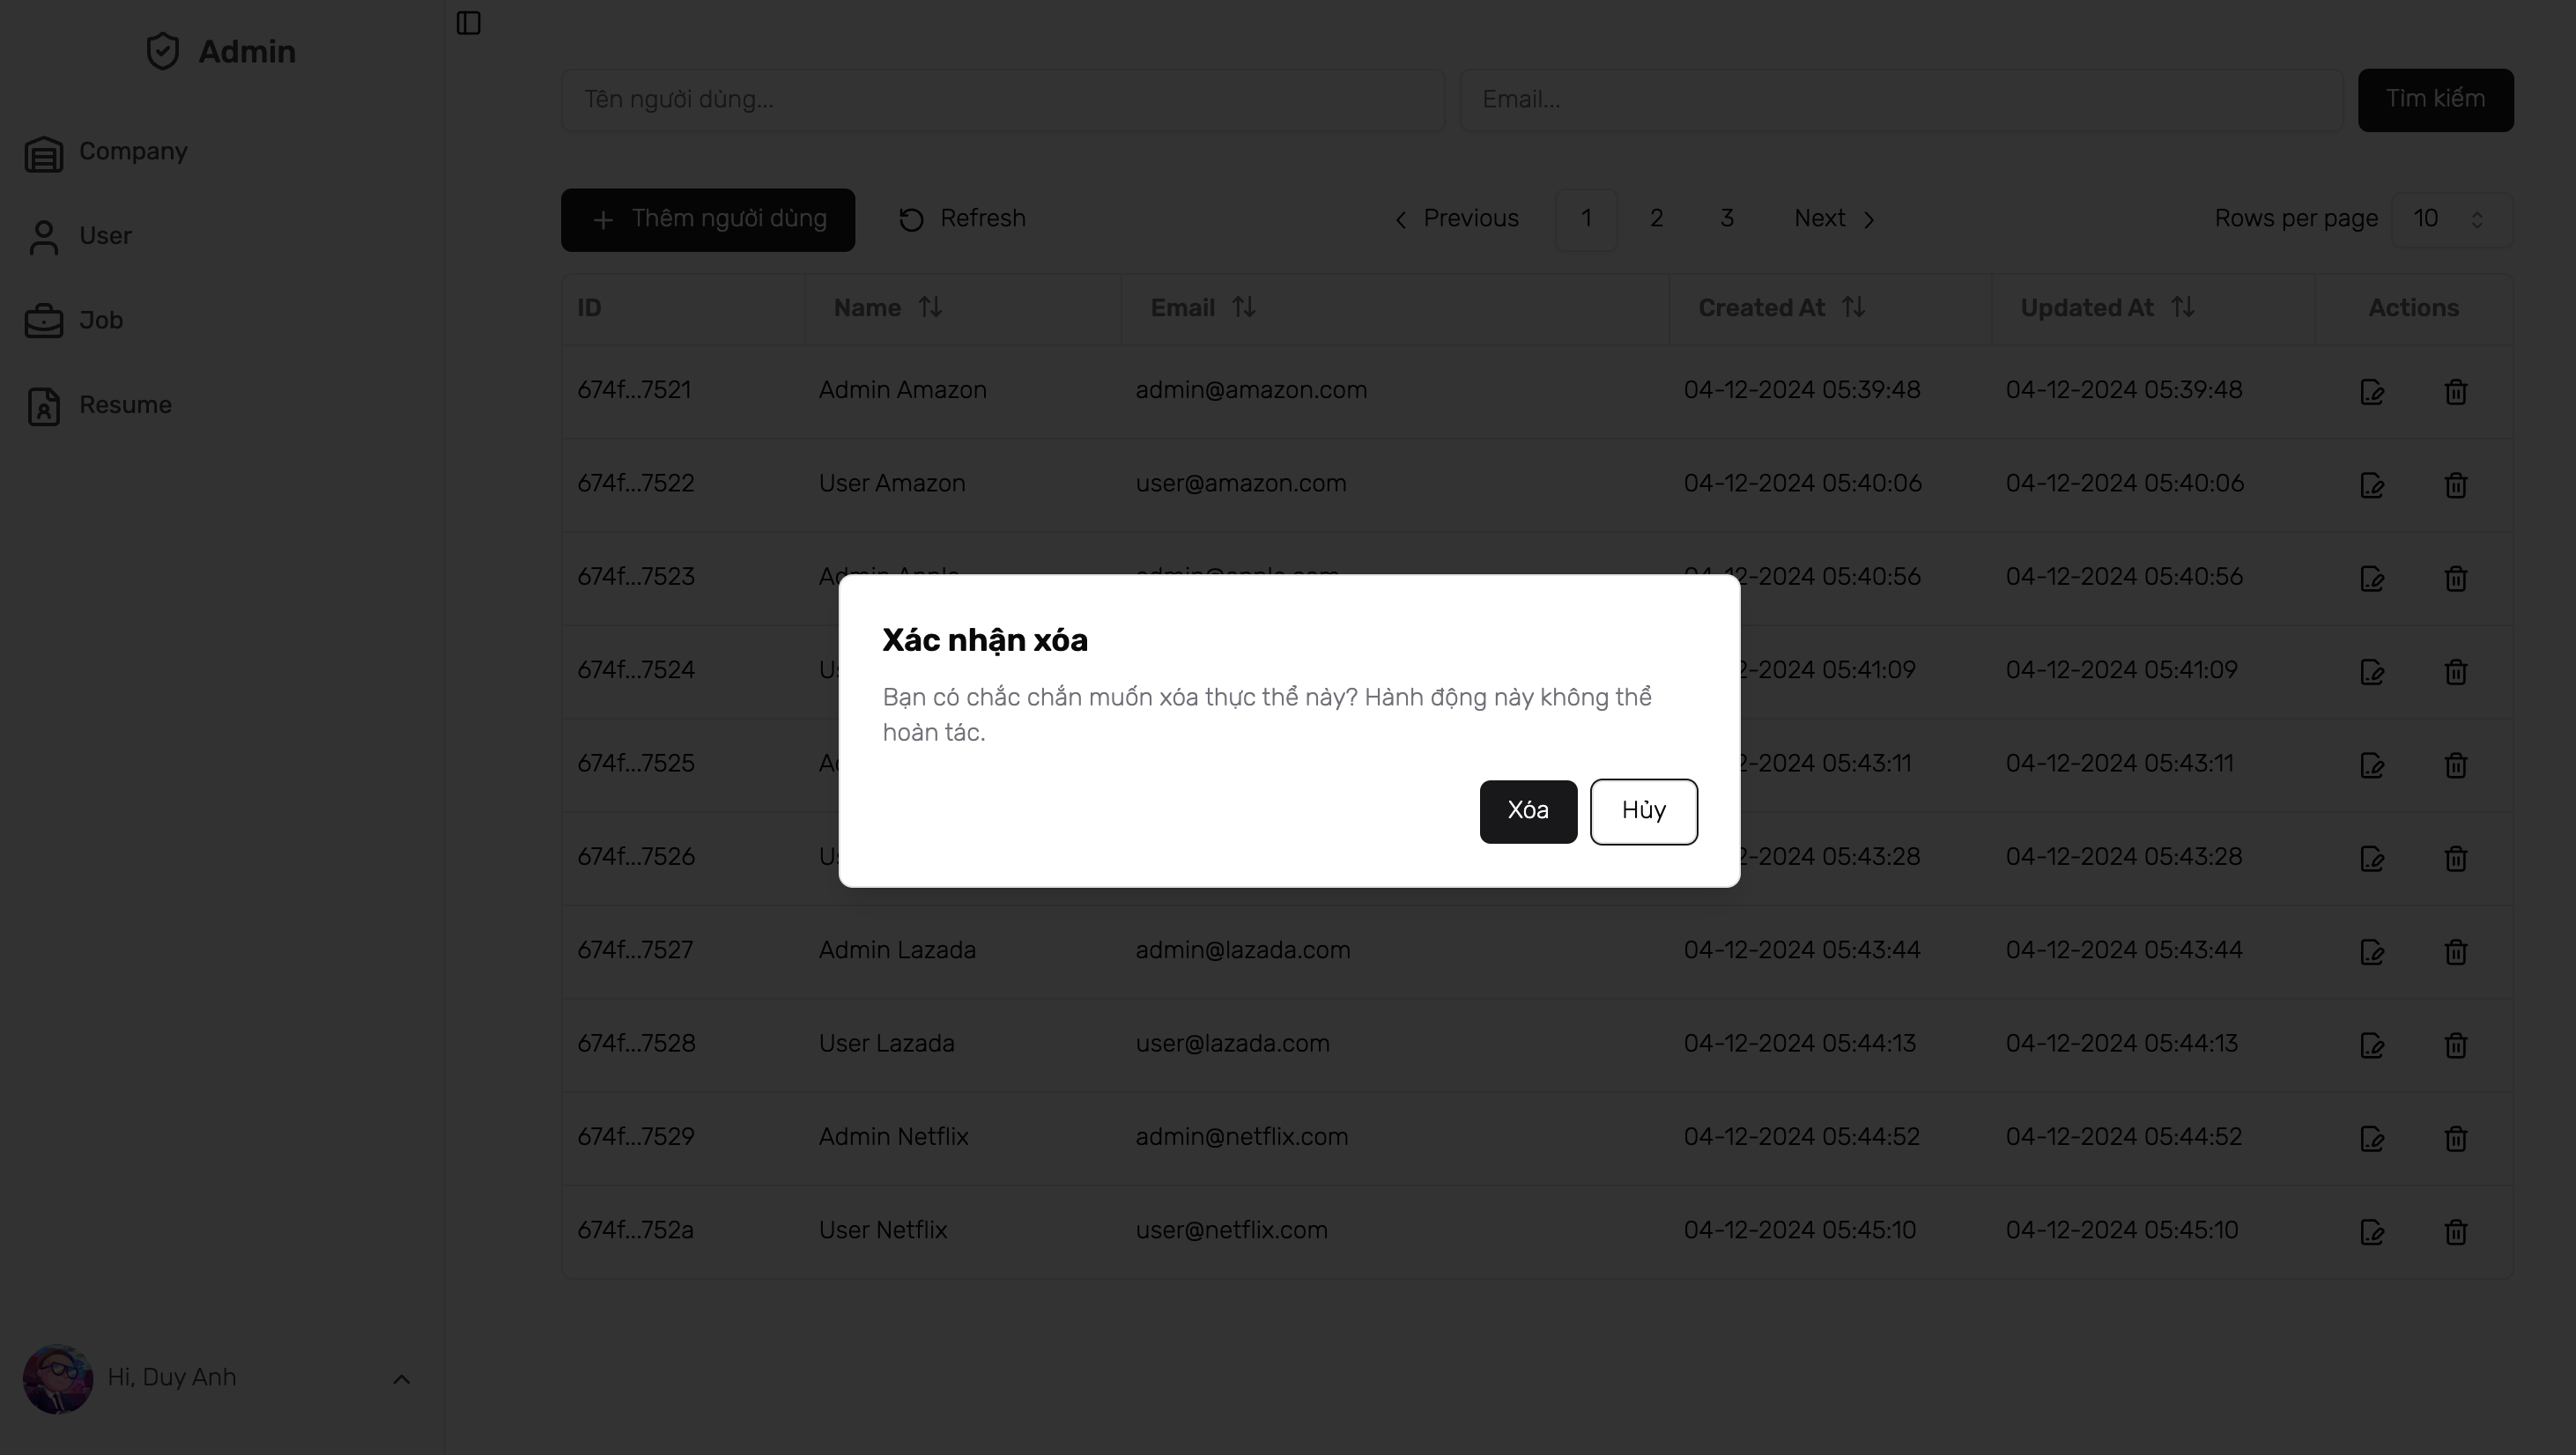
\includegraphics[width=\linewidth]{DBMS-Application/Images/delete-user.png}
        \caption{Trang quản lý người dùng - Xoá người dùng}
        \label{fig:enter-label}
    \end{figure}
\end{itemize}